\documentclass[tikz,border=6pt]{standalone}
\usepackage{amsmath}
\usepackage{newtxtext,newtxmath}
\usetikzlibrary{arrows.meta,calc,positioning}

\begin{document}
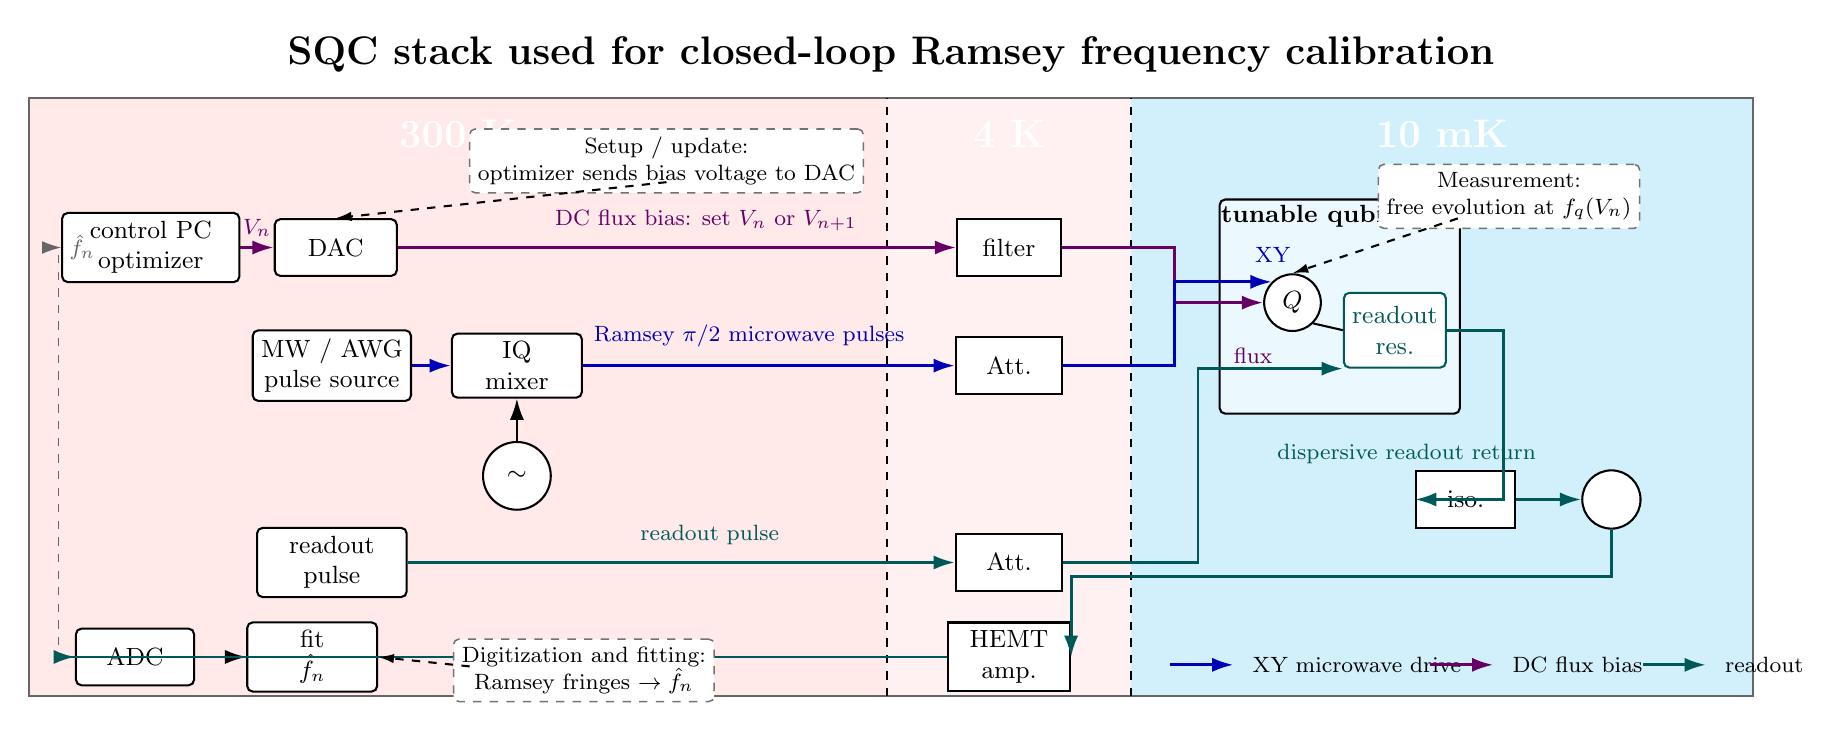
\begin{tikzpicture}[
  x=1cm,
  y=1cm,
  >=Latex,
  font=\small,
  line/.style={draw=black,line width=0.75pt},
  frame/.style={draw=black!60,line width=0.75pt},
  box/.style={line,fill=white,align=center,minimum height=0.72cm,inner sep=3pt},
  roundbox/.style={line,rounded corners=2pt,fill=white,align=center,minimum height=0.72cm,inner sep=3pt},
  chipbox/.style={line,rounded corners=2pt,fill=white,align=center,inner sep=3pt},
  xy/.style={draw=blue!72!black,line width=1.05pt},
  flux/.style={draw=violet!80!black,line width=1.05pt},
  ro/.style={draw=teal!70!black,line width=1.05pt},
  xyarr/.style={xy,-{Latex[length=2.7mm,width=1.8mm]}},
  fluxarr/.style={flux,-{Latex[length=2.7mm,width=1.8mm]}},
  roarr/.style={ro,-{Latex[length=2.7mm,width=1.8mm]}},
  blkarr/.style={line,-{Latex[length=2.7mm,width=1.8mm]}},
  callout/.style={draw=black!55,dashed,line width=0.55pt,rounded corners=2pt,fill=white,align=center,font=\footnotesize,inner sep=3pt},
  temp/.style={font=\bfseries\Large,text=white,align=center},
  labxy/.style={font=\footnotesize,text=blue!72!black,align=center},
  labflux/.style={font=\footnotesize,text=violet!80!black,align=center},
  labro/.style={font=\footnotesize,text=teal!70!black,align=center}
]

% ---------------------------------------------------------------------------
% Temperature zones, reference-figure style.
\fill[pink!35] (0.4,0.55) rectangle (11.3,8.15);
\fill[pink!22] (11.3,0.55) rectangle (14.4,8.15);
\fill[cyan!18] (14.4,0.55) rectangle (22.3,8.15);
\draw[frame] (0.4,0.55) rectangle (22.3,8.15);
\draw[black,dashed,line width=0.9pt] (11.3,0.55) -- (11.3,8.15);
\draw[black,dashed,line width=0.9pt] (14.4,0.55) -- (14.4,8.15);

\node[temp] at (5.85,7.70) {300 K};
\node[temp] at (12.85,7.70) {4 K};
\node[temp] at (18.35,7.70) {10 mK};
\node[font=\bfseries\Large] at (11.35,8.70)
  {SQC stack used for closed-loop Ramsey frequency calibration};

% ---------------------------------------------------------------------------
% 300 K classical control and sources.
\node[roundbox,minimum width=2.25cm] (ctrl) at (1.95,6.25) {control PC\\optimizer};
\node[roundbox,minimum width=1.55cm] (dac) at (4.30,6.25) {DAC};
\node[roundbox,minimum width=1.95cm] (mw) at (4.25,4.75) {MW / AWG\\pulse source};
\node[roundbox,minimum width=1.65cm] (iq) at (6.60,4.75) {IQ\\mixer};
\node[circle,line,minimum size=0.86cm,fill=white] (lo) at (6.60,3.35) {$\sim$};
\node[roundbox,minimum width=1.90cm] (roSrc) at (4.25,2.25) {readout\\pulse};
\node[roundbox,minimum width=1.50cm] (adc) at (1.75,1.05) {ADC};
\node[roundbox,minimum width=1.65cm] (fit) at (4.00,1.05) {fit\\$\hat f_n$};

\draw[fluxarr] (ctrl.east) -- node[above,font=\footnotesize,text=violet!80!black] {$V_n$} (dac.west);
\draw[xyarr] (mw.east) -- (iq.west);
\draw[blkarr] (lo.north) -- (iq.south);
\draw[blkarr] (adc.east) -- (fit.west);
\draw[black!60,dashed,-{Latex[length=2.4mm,width=1.6mm]}]
  (fit.west) -- (0.78,1.05) -- (0.78,6.25) --
  node[pos=0.45,right,font=\footnotesize] {$\hat f_n$} (ctrl.west);

% ---------------------------------------------------------------------------
% 4 K chain, deliberately minimal.
\node[box,minimum width=1.32cm] (fluxFilt) at (12.85,6.25) {filter};
\node[box,minimum width=1.35cm] (driveAtt) at (12.85,4.75) {Att.};
\node[box,minimum width=1.35cm] (roAtt) at (12.85,2.25) {Att.};
\node[box,minimum width=1.55cm] (hemt) at (12.85,1.05) {HEMT\\amp.};

% ---------------------------------------------------------------------------
% 10 mK chip and readout chain.
\node[chipbox,minimum width=3.05cm,minimum height=2.72cm,fill=cyan!8] (chip) at (17.05,5.50) {};
\node[font=\bfseries\small] at (17.05,6.65) {tunable qubit chip};
\node[circle,line,minimum size=0.72cm,fill=white] (qubit) at (16.45,5.55) {$Q$};
\node[chipbox,minimum width=1.15cm,minimum height=0.95cm,draw=teal!70!black,text=teal!70!black] (res) at (17.75,5.20)
  {readout\\res.};
\draw[line] (qubit.south east) -- (res.west);
\node[labxy] at (16.20,6.15) {XY};
\node[labflux] at (15.95,4.88) {flux};

\node[circle,line,minimum size=0.74cm,fill=white] (circ) at (20.50,3.05) {$\circlearrowright$};
\node[box,minimum width=1.26cm] (iso) at (18.65,3.05) {iso.};

% ---------------------------------------------------------------------------
% Three relevant signal paths.
% DC flux-bias path.
\draw[fluxarr] (dac.east) -- (fluxFilt.west);
\draw[fluxarr] (fluxFilt.east) -- ++(0.85,0) -- (14.95,6.25) |- (qubit.west);
\node[labflux,anchor=south] at (9.00,6.34) {DC flux bias: set $V_n$ or $V_{n+1}$};

% Ramsey microwave drive path.
\draw[xyarr] (iq.east) -- (driveAtt.west);
\draw[xyarr] (driveAtt.east) -- ++(0.95,0) -- (14.95,4.75) |- (qubit.north west);
\node[labxy,anchor=south] at (9.55,4.86) {Ramsey $\pi/2$ microwave pulses};

% Readout input path.
\draw[roarr] (roSrc.east) -- (roAtt.west);
\draw[roarr] (roAtt.east) -- ++(1.20,0) -- (15.25,2.25) |- (res.south west);
\node[labro,anchor=south] at (9.05,2.35) {readout pulse};

% Readout output path.
\draw[roarr] (res.east) -- ++(0.72,0) |- (iso.west);
\draw[roarr] (iso.east) -- (circ.west);
\draw[roarr] (circ.south) -- ++(0,-0.60) -| (hemt.east);
\draw[roarr] (hemt.west) -- ++(-1.20,0) -- (0.75,1.05) -- (adc.west);
\node[labro,anchor=south] at (17.90,3.38) {dispersive readout return};

% ---------------------------------------------------------------------------
% Operation annotations.
\node[callout] at (8.50,7.35) {Setup / update:\\optimizer sends bias voltage to DAC};
\draw[line,dashed,-{Latex[length=2.0mm,width=1.2mm]}] (8.50,7.08) -- (dac.north);

\node[callout] at (19.20,6.90) {Measurement:\\free evolution at $f_q(V_n)$};
\draw[line,dashed,-{Latex[length=2.0mm,width=1.2mm]}] (18.55,6.62) -- (qubit.north);

\node[callout] at (7.45,0.88) {Digitization and fitting:\\Ramsey fringes $\rightarrow \hat f_n$};
\draw[line,dashed,-{Latex[length=2.0mm,width=1.2mm]}] (6.00,0.93) -- (fit.east);

% Legend
\draw[xyarr] (14.90,0.95) -- ++(0.80,0);
\node[anchor=west,font=\footnotesize] at (15.82,0.95) {XY microwave drive};
\draw[fluxarr] (18.20,0.95) -- ++(0.80,0);
\node[anchor=west,font=\footnotesize] at (19.12,0.95) {DC flux bias};
\draw[roarr] (20.90,0.95) -- ++(0.80,0);
\node[anchor=west,font=\footnotesize] at (21.82,0.95) {readout};

\end{tikzpicture}
\end{document}
